\documentclass[12pt]{article}
\usepackage[hidelinks]{hyperref}    
\usepackage[all]{hypcap}
\usepackage{graphicx}
\usepackage{circuitikz}
\graphicspath{{../images/}} % imposta path per trovare le immagini, i .. significano "la dir precedente"
\author{Andrea Malvezzi}
\title{\textbf{Architettura degli Elaboratori~-~Porte logiche e circuiti combinatori}}  % textbf = testo bold
\date{26 Settembre, 2024}
\author{Andrea Malvezzi}
\begin{document}
\maketitle
\pagebreak
\tableofcontents
\pagebreak
\section{Algebra di Boole}
\subsection{Espressioni booleane}
Un'espressione booleana si costruisce usando:
\begin{itemize}
    \item 0 e 1 (False e True);
    \item gli operatori booleani (o logici);
    \item delle variabili sempre con valore 0 oppure 1.
\end{itemize}
\subsection{Proprietà dell'algebra di Boole}
Nella tabella seguente sono presenti delle equivalenze per descrivere le proprietà dell'algebra di Boole.
\begin{figure}[!htb]
    \centering
    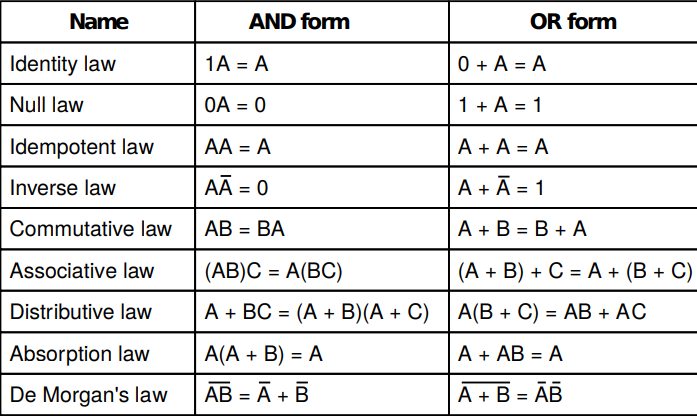
\includegraphics[width=1\textwidth, height=.7\textheight,keepaspectratio]{porte_logiche/properties_boole.png} % essenzialmente resiza l'immagine
    \begin{center}
        \caption{\label{fig:properties_boolean_algebra}Una visualizzazione delle proprietà dell'algebra di Boole.} % label fuori da caption spesso non va, mettilo dentro
    \end{center}
\end{figure}
\pagebreak
\subsubsection{La legge di De Morgan}
La più importante tra le leggi presentate è sicuramente quella di De Morgan,\\
in quanto permette di passare da una colonna della tabella all'altra in modo semplice e veloce.
\subsubsection{Esempio di applicazione della legge di De Morgan}
\begin{itemize}
    \item Per cominciare, scriviamo la OR form della legge inversa: $A + \overline{A} = 1$;
    \item Seguentemente occorre pensare a com'è scritta l'espressione: siamo\\davanti ad una OR tra due variabili A, di cui una negata, il tutto pari ad 1;
    \item Ora osserviamo la legge di De Morgan nella forma OR. Questa afferma quanto segue: La negazione di una OR equivale ad una AND con entrambi gli input negati;
    \item Applichiamo quindi De Morgan: $\overline{A} + A = 1$ diventerà $\overline{A\overline{A}} = \overline{1}$, ovvero $\overline{A}A = 0$.
\end{itemize}
Ed ecco mostrato come passare da un lato all'altro della tabella tramite la formula di De Morgan.
\subsection{Formula canonica}
Una funzione booleana si può definire attraverso un'espressione basata solamente sulla AND, la OR e la NOT.\\
Inoltre, una funzione booleana è esprimibile in una forma detta "canonica". Per ricavarla occorre:
\begin{itemize}
    \item identificare tutte le combinazioni per cui la funzione in esame è vera (queste son dette \textbf{mintermini});
    \item fare la OR dei mintermini trovati;
\end{itemize}
\pagebreak
\subsubsection{Esempio di formula canonica}
Analizziamo la seguente tabella:
\begin{figure}[!htb]
    \centering
    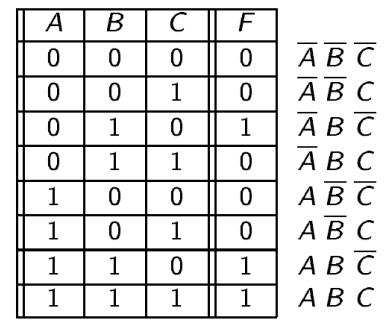
\includegraphics[width=.7\textwidth, height=.7\textheight,keepaspectratio]{porte_logiche/canonica.png} % essenzialmente resiza l'immagine
    \begin{center}
        \caption{\label{fig:canonica_esempio}Nella tabella presentata si hanno 3 mintermini: $\overline{A}B\overline{C}$, $AB\overline{C}$, $ABC$.} % label fuori da caption spesso non va, mettilo dentro
    \end{center}
\end{figure}\\
Ora dobbiamo fare la OR tra i 3 mintermini trovati precedentemente:
\begin{center}
    $\overline{A}B\overline{C} + AB\overline{C} + ABC$
\end{center}
Questa espressione equivale alla forma canonica della funzione studiata.
\pagebreak
\section{I transistor}
Un transistor è un dispositivo a 3 connettori: \textbf{collettore}, \textbf{emettitore} e \textbf{base}.\\
Quando non c'è tensione sulla base, il componente agisce come una resistenza infinita tra emettitore e collettore.\\
In caso contrario, si comporta da conduttore ideale.
\begin{figure}[!htb]
    \centering
    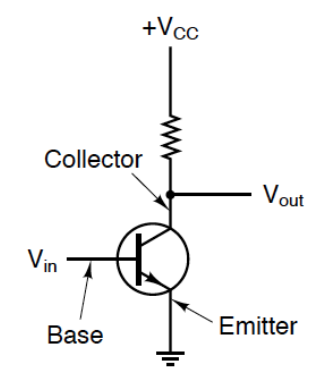
\includegraphics[width=.7\textwidth, height=.7\textheight,keepaspectratio]{porte_logiche/transistor_not_ex.png} % essenzialmente resiza l'immagine
    \begin{center}
        \caption{\label{fig:transistor_not_esempio}Esempio di porta NOT realizzata con transistor.} % label fuori da caption spesso non va, mettilo dentro
    \end{center}
\end{figure}
\subsection{La porta NOT realizzata tramite transistor}
La porta NOT della figura (\ref{fig:transistor_not_esempio}) funziona nella seguente maniera:
\begin{itemize}
    \item quando l'ingresso \textit{V\textsubscript{in}} è \textit{alto}, la corrente \textit{V\textsubscript{cc}} attraversa il transistor e lascia \textit{V\textsubscript{out}} basso (Input 1, output 0);
    \item quando l'ingresso \textit{V\textsubscript{in}} è \textit{basso}, la corrente \textit{V\textsubscript{cc}} non riesce ad attraversare il transistor, il quale agisce da resistenza infinita, passando quindi per \textit{V\textsubscript{out}}, il quale diventa alto (Input 0, output 1).
\end{itemize}
\subsection{La porta NAND realizzata tramite transistor}
Per realizzare una porta NAND occorranno due transistor:
\begin{figure}[!htb]
    \centering
    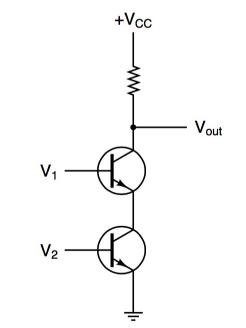
\includegraphics[width=.5\textwidth, height=.4\textheight,keepaspectratio]{porte_logiche/transistor_nand_ex.png} % essenzialmente resiza l'immagine
    \begin{center}
        \caption{\label{fig:transistor_nand_esempio}Esempio di porta NAND realizzata con 2 transistor.} % label fuori da caption spesso non va, mettilo dentro
    \end{center}
\end{figure}\\
Il funzionamento della porta logica in figura è simile a quello della NOT in (\ref{fig:transistor_not_esempio}): 
\begin{itemize}
    \item quando l'alimentazione di entrambi i transistor è alta, \textit{V\textsubscript{out}} non riceverà corrente (0);
    \item quando uno dei due transistor NON sarà alimentato, \textit{V\textsubscript{out}} sarà alimentato (1).
\end{itemize}
\section{La porta XOR}
\begin{circuitikz} \draw(0, 2) node[xor port, number inputs=2](myxor){}
    (myxor.in 1) node[anchor=east]{A}
    (myxor.in 2) node[anchor=east]{B}
    (myxor.out) node[anchor=west]{Output}
    ;
\end{circuitikz}
\hfill
\begin{tabular}{|| c c | c ||}
    \hline
    A & B & Output\\
    \hline
    0 & 0 & 0\\
    \hline
    0 & 1 & 1\\
    \hline
    1 & 0 & 1\\
    \hline
    1 & 1 & 0\\
    \hline
\end{tabular}\\\\
La funzione logica XOR restituisce VERO quando \underline{soltanto} uno dei due valori in ingresso è VERO.\\
Inoltre, la funzione logica XOR si può rappresentare con la seguente forma canonica:
\begin{equation}
    XoR(a, b) = Or(And(a, NOT(b)), And(Not(a),b)) = (a \cdot \overline{b}) + (\overline{a} \cdot b) \label{canon: xor}
\end{equation}
\section{Array logici programmabili (PLA)}
Sono circuiti universali precostituiti. Sono composti da una porta AND usata per confrontare tra loro i valori in input, e precisamente se ne ha una per mintermine. Queste porte saranno collegate ad una stessa porta OR.
\begin{figure}[!htb]
    \centering
    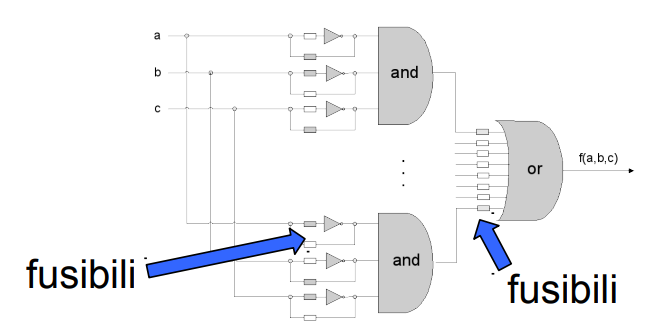
\includegraphics[width=.5\textwidth, height=.4\textheight,keepaspectratio]{porte_logiche/PLA.png} % essenzialmente resiza l'immagine
    \begin{center}
        \caption{\label{fig:PLA}Esempio di PLA tra 2 mintermini, con 3 valori in input.} % label fuori da caption spesso non va, mettilo dentro
    \end{center}
\end{figure}\\
\pagebreak
\section{Implementare una funzione logica}
\subsection{Dalla forma canonica all'implementazione}\label{sec:implem_canonica}
Per implementare una funzione logica (ovvero per realizzarla mediante porte logiche) occorre innanzitutto studiarne la tabella di verità, in modo da ricavarne la forma canonica.\\
Ad esempio, avendo la seguente tabella di verità:\\
\begin{center}
    \begin{tabular}{|| c c c | c ||}
        \hline
        A & B & SEL & OUT\\
        \hline
        0 & 0 & 0 & 0\\
        \hline
        0 & 0 & 1 & 0\\
        \hline
        0 & 1 & 0 & 0\\
        \hline
        0 & 1 & 1 & 1\\
        \hline
        1 & 0 & 0 & 1\\
        \hline
        1 & 0 & 1 & 0\\
        \hline
        1 & 1 & 0 & 1\\
        \hline
        1 & 1 & 1 & 1\\
        \hline
    \end{tabular}
\end{center}
Occorrerà identificare tutti i mintermini della funzione ed effettuare una OR tra questi, ovvero:
\begin{itemize}
    \item $\overline{A} \cdot B \cdot SEL$
    \item $A \cdot \overline{B} \cdot \overline{SEL}$
    \item $A \cdot B \cdot \overline{SEL}$
    \item $A \cdot B \cdot SEL$
\end{itemize}
Ed infine:
\[
    (\overline{A} \cdot B \cdot SEL) + (A \cdot \overline{B} \cdot \overline{SEL}) + (A \cdot B \cdot \overline{SEL}) + (A \cdot B \cdot SEL)
\]
Ora che la forma canonica è nota, si può procedere a realizzare il circuito:
\begin{circuitikz} \draw
    (0, 6) node[and port, number inputs=3](first_and){}
    (first_and.in 1) node[anchor=east]{$\overline{A}$}
    (first_and.in 2) node[anchor=east]{B}
    (first_and.in 3) node[anchor=east]{SEL}
    (0, 4) node[and port, number inputs=3](second_and){}
    (second_and.in 1) node[anchor=east]{A}
    (second_and.in 2) node[anchor=east]{$\overline{B}$}
    (second_and.in 3) node[anchor=east]{$\overline{SEL}$}
    (0, 2) node[and port, number inputs=3](third_and){}
    (third_and.in 1) node[anchor=east]{A}
    (third_and.in 2) node[anchor=east]{B}
    (third_and.in 3) node[anchor=east]{$\overline{SEL}$}
    (0, 0) node[and port, number inputs=3](fourth_and){}
    (fourth_and.in 1) node[anchor=east]{A}
    (fourth_and.in 2) node[anchor=east]{B}
    (fourth_and.in 3) node[anchor=east]{SEL}
    (4, 3) node[or port, number inputs=4](or){}
    (or.out) node[anchor=west]{Output}
    (first_and.out) -- (or.in 1)
    (second_and.out) -- (or.in 2)
    (third_and.out) -- (or.in 3)
    (fourth_and.out) -- (or.in 4)
    ;
    \node at (first_and.bin 1) [ocirc, left]{};
    \node at (second_and.bin 2) [ocirc, left]{};
    \node at (second_and.bin 3) [ocirc, left]{};
    \node at (third_and.bin 3) [ocirc, left]{};
\end{circuitikz}
\subsection{Semplificare un circuito logico}
Per semplificare un circuito logico si può utilizzare un potente strumento chiamato \textbf{Mappa di Karnaugh}, o \textbf{K-map}.\\
Ecco come realizzare una mappa di Karnaugh:
\subsubsection{Definire le variabili}
Per realizzare una K-map occorrerà identificare le variabili usate nella funzione logica di cui si sta semplificando la tabella di verità.\\
In base al numero di variabili scelte ($n$), si avranno $2^n$ celle nella tabella.
\subsubsection{Disegnare la mappa}
La K-map è una griglia dove, in base al numero di variabili cambia il numero di celle.\\
Ad esempio, per 2 variabili, si avranno $2^2 = 4$ celle:
\begin{center}
    \begin{tabular}{|| c | c c ||}
        \hline
        A/B & 0 & 1\\
        \hline
        0 & $\dots$ & $\dots$\\
        1 & $\dots$ & $\dots$\\
        \hline
    \end{tabular}
\end{center}
Con l'aumentare del numero delle variabili, invece la cosa cambierà leggermente.\\
Ad esempio, per 3 variabili:
\begin{center}
    \begin{tabular}{|| c | c c c c ||}
        \hline
        A/BC & 00 & 01 & 11 & 10\\
        \hline
        0 & $\dots$ & $\dots$ & $\dots$ & $\dots$\\
        \hline
        1 & $\dots$ & $\dots$ & $\dots$ & $\dots$\\
        \hline  
    \end{tabular}
\end{center}
Mentre con 4:
\begin{center}
    \begin{tabular}{|| c | c c c c ||}
        \hline
        AD/BC & 00 & 01 & 11 & 10\\
        \hline
        00 & $\dots$ & $\dots$ & $\dots$ & $\dots$\\
        \hline
        01 & $\dots$ & $\dots$ & $\dots$ & $\dots$\\
        \hline
        11 & $\dots$ & $\dots$ & $\dots$ & $\dots$\\
        \hline
        10 & $\dots$ & $\dots$ & $\dots$ & $\dots$\\
        \hline
    \end{tabular}
\end{center}
Inoltre è importante notare come le coppie (00, 01, 10, 11, $\dots$) siano arbitrariamente posizionate: l'obiettivo è creare gruppi di 1 posizionati adiacenti verticalmente, orizzontalmente o in modo toroidale.
\subsubsection{Riempire la mappa}
Ora bisogna riempire la mappa creata mettendo 1 dove la combinazione di Input restituisce 1 e 0 nelle altre celle.
Ad esempio, prendendo la funzione presentata in (\ref{sec:implem_canonica}):
\begin{center}
    \begin{tabular}{|| c | c c c c ||}
        \hline
        A/B(SEL) & 00 & 01 & 11 & 10 \\
        \hline
        0 & 0 & 0 & 1 & 0 \\
        \hline
        1 & 1 & 0 & 1 & 1 \\
        \hline
    \end{tabular}
\end{center}
Ora abbiamo due gruppi di 1:
\begin{itemize}
    \item A = 0 con B, SEL = 11 \& A = 1 con B, SEL = 11 (verticalmente);
    \item A = 1 con B, SEL = 00 \& A = 1 con B, SEL = 10 (toroidalmente);
\end{itemize}
\subsubsection{Funzione semplificata}
In base ai raggruppamenti effettuati nella sezione precedente, ora possiamo scrivere la forma canonica semplificata della funzione, ovvero:
\[
    B \cdot SEL + A \cdot \overline{SEL}
\]
\pagebreak
\subsubsection{Come prendere le lettere?}
Ma perché? Per capire come determinare le lettere in base ai raggruppamenti fatti, osserviamo la tabella precedentemente presentata.\\
In essa è possibile notare, per ogni raggruppamento, come alcune lettere cambino di valore (da 1 a 0 e viceversa), mentre altre rimangano costanti.\\
Per ogni raggruppamento occorrerà prendere tutte le lettere rimaste costanti per l'intero gruppo creato e negare quelle rimaste a 0.
Quindi, nell'esempio presentato:
\begin{center}
    \begin{tabular}{|| c | c c c c ||}
        \hline
        A/B(SEL) & 00 & 01 & \colorbox{green}{11} & 10 \\
        \hline
        0 & 0 & 0 & \colorbox{cyan}{1} & 0 \\
        \hline
        1 & 1 & 0 & \colorbox{cyan}{1} & 1 \\
        \hline
    \end{tabular}
\end{center}
Come visibile, nel raggruppamento verticale scelto le uniche due lettere a rimanere costanti sono B e SEL.
Per quanto riguarda il raggruppamento toroidale, invece:
\begin{center}
    \begin{tabular}{|| c | c c c c ||}
        \hline
        A/B(SEL) & 00 & 01 & 11 & 10 \\
        \hline
        0 & 0 & 0 & 1 & 0 \\
        \hline
        \colorbox{green}{1} & \colorbox{cyan}{1} & 0 & 1 & \colorbox{cyan}{1} \\
        \hline
    \end{tabular}
\end{center}
\end{document}